\begin{figure*}[!ht]
 \centering
 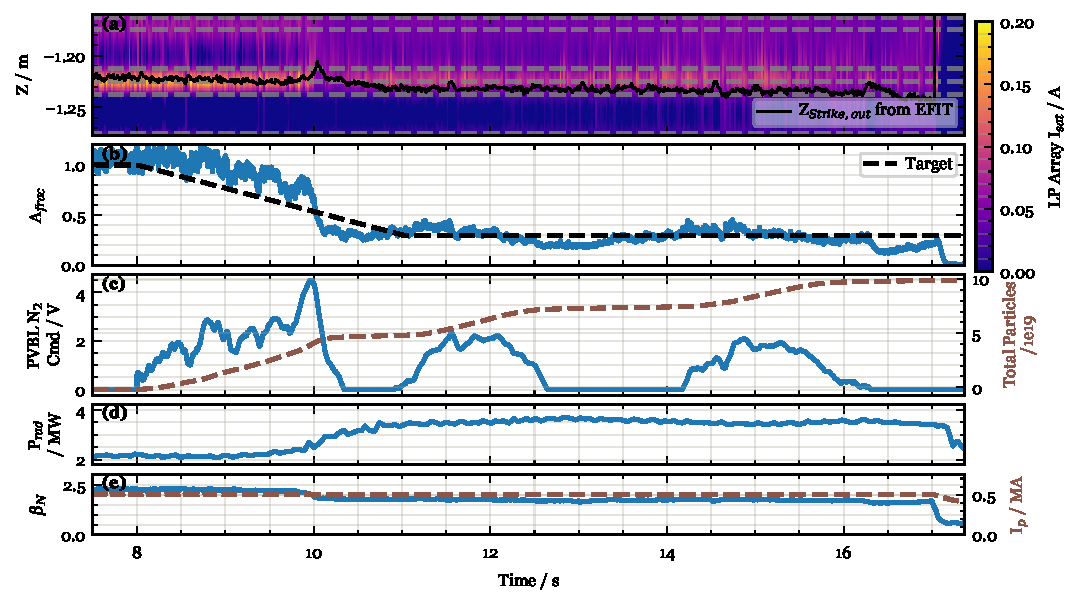
\includegraphics[width=\textwidth]{figures/DetCtrl_2D_35857.pdf}
 \caption{
Detachment control shot \#35857 using \Afrac controller.
(a) Shows the measured ion saturation current by realtime \ac{LP} array at locations marked by grey dashed lines.
The data has been interpolated spatially using cubic spline interpolation.
The black curve shows the post-shot calculated strike point position on outer divertor using EFIT.
(b) Shows the \Afrac calculated from peak value among the \ac{LP}  array.
The dashed black line shows the target provided to the controller to follow.
(c) Left axis: Shows the N$_2$ gas command steps sent for system identification.
Right axis: Shows the cummulative N$_2$ gas particles injected into the vessel.
(d) Total radiated power measured by \ac{IRVB}.
(e) Left axis: Shows $\beta_n$.
Right axis: Shows the plasma current (I$_p$).
}
 \label{fig:detctrl_afrac}
\end{figure*}